\chapter{Estado del Arte y Marco Teórico}
\label{chap:estado_arte}

\lettrine{P}{ara} comprender adecuadamente las decisiones arquitectónicas y técnicas tomadas en este proyecto, es fundamental contextualizar los conceptos teóricos subyacentes. Este capítulo describe los fundamentos de la Inteligencia de Negocios y las herramientas ETL que sustentan el Datamart desarrollado.

\section{Inteligencia de Negocios y Data Warehousing}
La Inteligencia de Negocios (\textit{Business Intelligence} o BI) comprende el conjunto de metodologías, aplicaciones y tecnologías que permiten reunir, depurar y transformar datos de sistemas transaccionales en información estructurada, para su explotación directa o para su análisis y conversión en conocimiento.

En el ámbito educativo, el BI permite a los centros pasar de un modelo reactivo a uno proactivo, identificando patrones y tendencias en el rendimiento de los alumnos antes de que se consolide el fracaso escolar.

\subsection{Metodología de Ralph Kimball}
Para el diseño del repositorio de datos se ha optado por la metodología ascendente o \textit{Bottom-Up} propuesta por Ralph Kimball \cite{Kimball_DWH}. A diferencia de enfoques transaccionales clásicos, Kimball propone construir el almacén de datos (Data Warehouse) a partir de la integración de diferentes \textit{Datamarts} temáticos.

Un Datamart es un subconjunto orientado a una área específica (en este caso, la orientación y prevención del abandono escolar). La estructura central de esta metodología es el modelo dimensional, habitualmente implementado mediante esquemas en estrella (ver Figura \ref{fig:star_schema_concept}). Para comprender este diseño, es esencial entender dos conceptos arquitectónicos clave:

\begin{itemize}
    \item \textbf{Modelo en Estrella:} Consiste en separar radicalmente la información en dos tipos de tablas. En el centro de la "estrella" se sitúan las \textit{Tablas de Hechos} (\textit{Fact Tables}), que almacenan eventos medibles y cuantitativos (por ejemplo, las calificaciones o el riesgo de abandono). Alrededor, conectadas directamente a la tabla de hechos, orbitan las \textit{Tablas de Dimensiones} (\textit{Dimension Tables}), que contienen el contexto descriptivo de esos eventos (el "quién", "cuándo", "dónde" y "qué": estudiante, tiempo, centro, curso).
    \item \textbf{Desnormalización Intencionada:} Mientras que las bases de datos operativas tradicionales (OLTP) aplican la "normalización" (dividir los datos en múltiples tablas para evitar redundancias y proteger la escritura), los Datamarts (OLAP) hacen exactamente lo contrario. Se aplica la \textit{desnormalización}, es decir, se admite la redundancia de datos (aplanando jerarquías como "Ciclo $\rightarrow$ Especialidad $\rightarrow$ Curso" en una sola tabla) con el objetivo de reducir drásticamente las operaciones matemáticas de cruce (JOINs). Esto permite que las consultas analíticas sobre grandes volúmenes de datos sean extremadamente rápidas para alimentar cuadros de mando.
\end{itemize}

\begin{figure}[htbp]
    \centering
    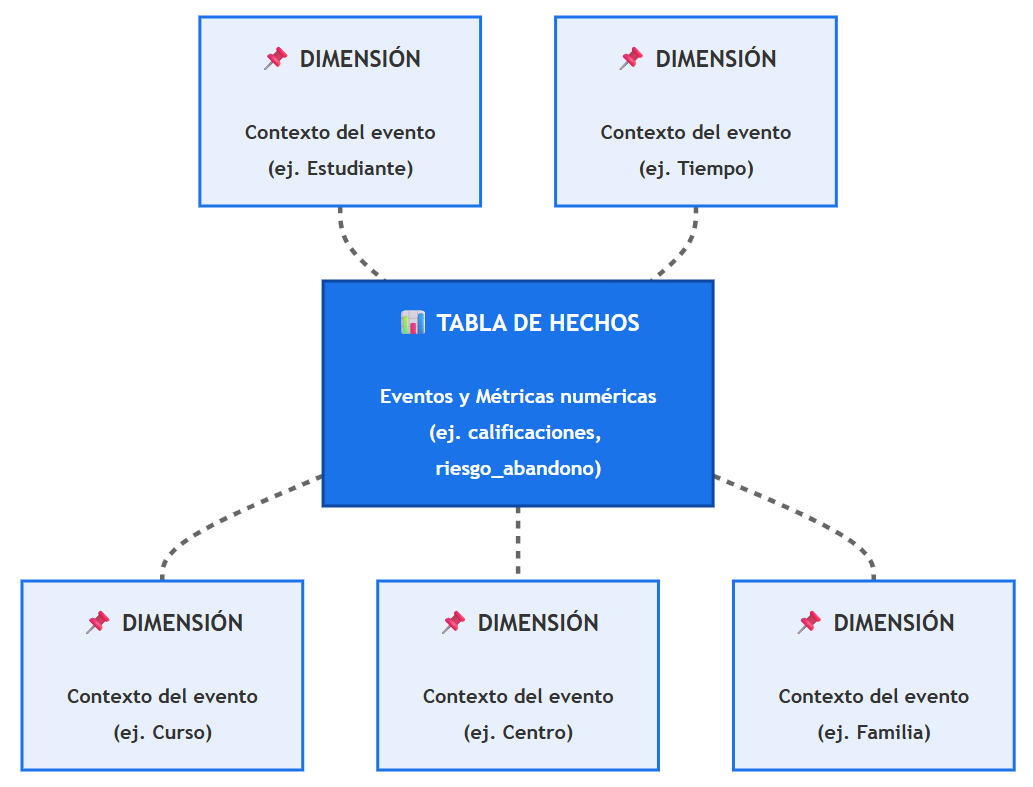
\includegraphics[width=0.8\textwidth]{imaxes/star_schema.png}
    \caption{Esquema conceptual de un modelo en estrella.}
    \label{fig:star_schema_concept}
\end{figure}

\section{Procesos ETL y Apache Hop}
Los procesos ETL (Extracción, Transformación y Carga) son el motor de cualquier sistema BI. Son los encargados de extraer los datos de las fuentes originales, aplicarles reglas de limpieza, filtrado y transformación, y finalmente cargarlos en el Datamart dimensional.

\subsection{Elección de Apache Hop}
Apache Hop (\textit{Hop Orchestration Platform}) \cite{Apache_Hop} es una plataforma moderna de ingeniería de datos y orquestación. Nace como una bifurcación (\textit{fork}) de Pentaho Data Integration (PDI), con el objetivo de modernizar su arquitectura, mejorar su integración con entornos de contenedores y facilitar su uso a través de una interfaz de usuario web (\textit{Hop Web}).

La elección de Apache Hop frente a otras herramientas del mercado se fundamenta en su curva de aprendizaje, su modelo visual \textit{drag-and-drop} (ver Figura \ref{fig:apache_hop_ui}) y, especialmente, su excelente soporte para la ejecución nativa en contenedores Docker, lo cual encaja perfectamente con la arquitectura diseñada para este proyecto.

\begin{figure}[htbp]
    \centering
    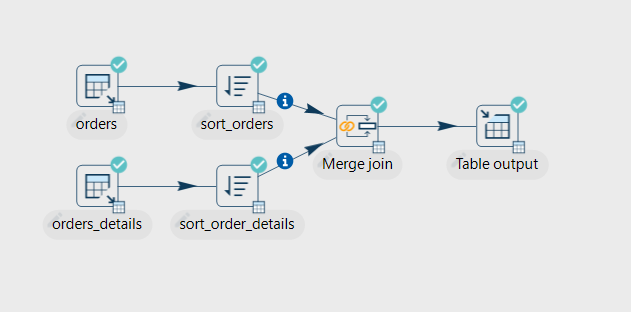
\includegraphics[width=1\textwidth]{imaxes/apache_hop_ui.png}
    \caption{Interfaz de usuario de Apache Hop.}
    \label{fig:apache_hop_ui}
\end{figure}
